\chapter{Experimental setup and hardware configuration}
\label{chap:experimental-setup-hardware-config}

This chapter describes the experimental setup and hardware configuration developed to validate the LINKU stereo vision system under controlled laboratory conditions.
\\\\
The experimental framework was designed to progressively reproduce the principal optical conditions associated with orbital tether observation while maintaining controlled and repeatable image acquisition. Particular emphasis was placed on reproducing low-texture environments, dark backgrounds, directional high-contrast illumination, and sub-pixel tether visibility conditions.
\\\\
Unlike conventional terrestrial stereo vision validation platforms, the proposed setup was specifically adapted for the observation of thin tether-like structures operating under conditions where environmental texture becomes limited and radiometric effects increasingly dominate the apparent image response.

\begin{figure}[!ht]
    \centering
    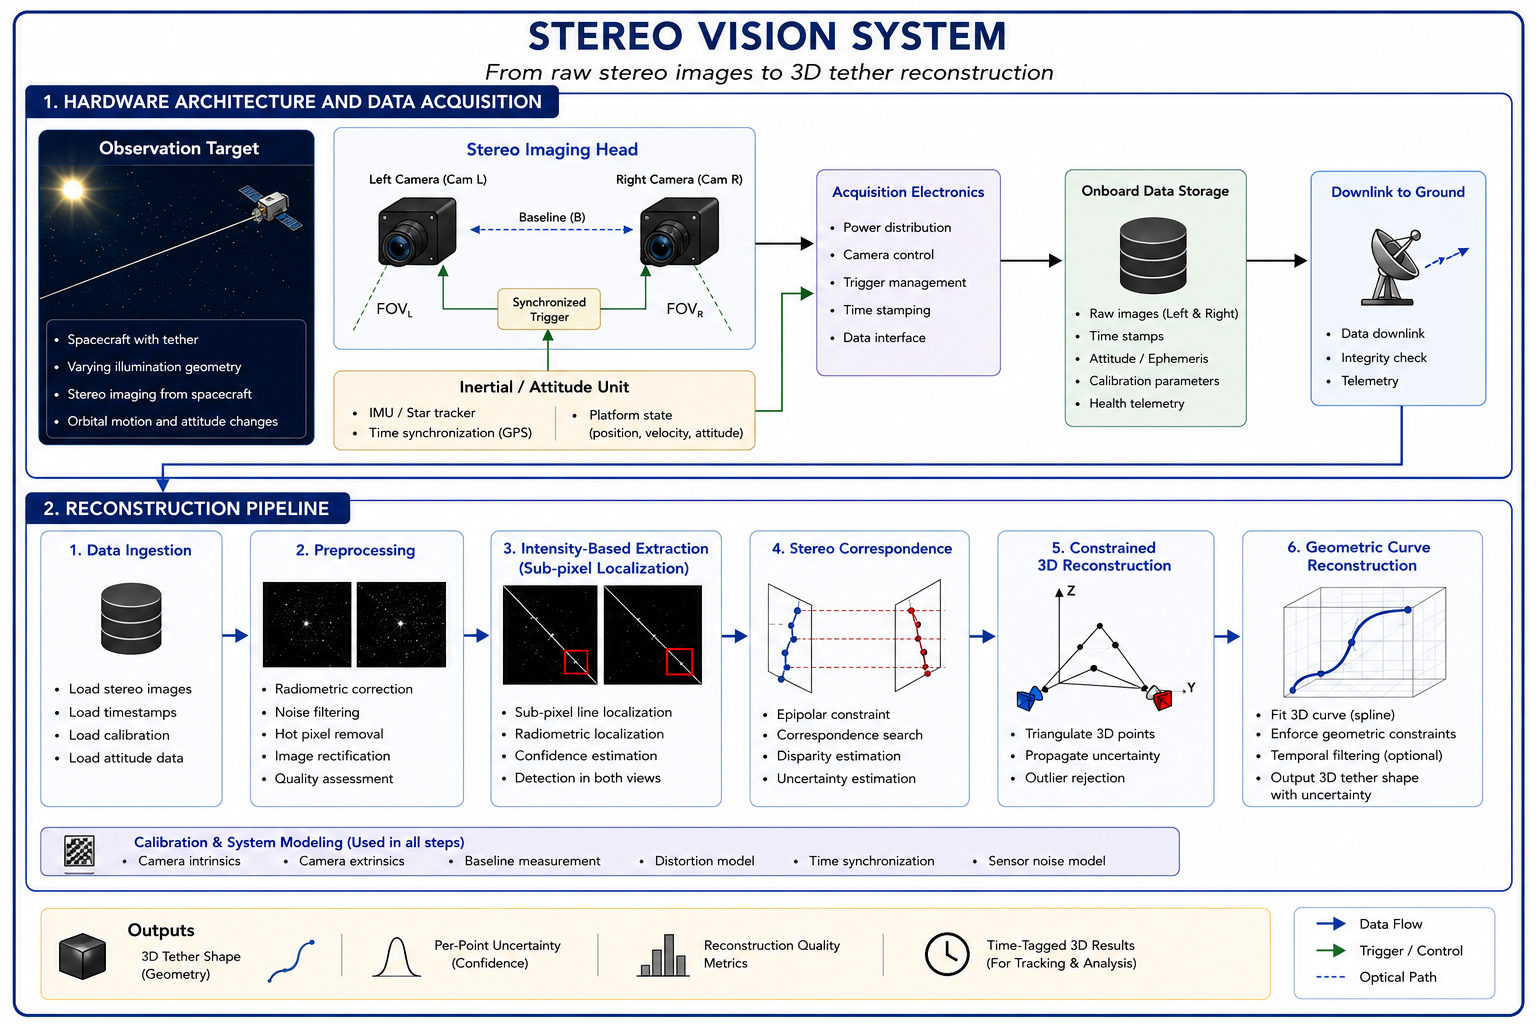
\includegraphics[width=\textwidth]{Images/Figure 5.1.png}
    \caption[Stereo vision system architecture and reconstruction pipeline.]{Stereo vision system architecture and reconstruction pipeline.}
    \label{fig:figure5.1}
\end{figure}

The experimental configuration was organized to support two principal validation objectives. First, it provides a controlled baseline for evaluating conventional feature-based photogrammetry under progressively constrained visual conditions. Second, it enables controlled evaluation of the geometry-driven stereo reconstruction stages introduced in Phase II under orbital-like imaging conditions. Figure \ref{fig:figure5.1} provides an overview of the LINKU stereo vision system considered throughout this chapter. The diagram summarizes the hardware architecture responsible for stereo image acquisition, the geometry-driven reconstruction pipeline, and the principal outputs generated during tether reconstruction. This system-level representation serves as a reference framework for the experimental validation activities described in the following sections.

Accordingly, the chapter is organized into two principal blocks:

\section{Hardware architecture and data acquisition}
\label{sec:Hardware-architecture-data-acquisition}

The imaging system consists of a stereo pair of synchronized image sensors interfaced with a centralized processing and acquisition platform. The architecture was designed to emulate the operational principles of the proposed flight stereo vision system while maintaining sufficient flexibility for laboratory characterization and optical testing.
\\\\
Particular attention was placed on optical repeatability, geometric stability, synchronization consistency, and configurable imaging conditions.
\\\\
The hardware platform enables controlled evaluation of stereo correspondence behavior, disparity generation, sub-pixel tether visibility, and geometric reconstruction stability under progressively constrained orbital-like optical conditions.

\subsection{Camera sensors and optics}
\label{sec:camera_sensors}
The stereo imaging system was implemented using two Raspberry Pi High Quality Cameras based on the Sony IMX477 image sensor. The sensor provides a native resolution of $4056 \times 3040$ pixels (12.3 MP), a pixel pitch of $1.55~\mu\mathrm{m}$, and a sensor width of $6.287~\mathrm{mm}$. These characteristics provide sufficient spatial sampling capability for the tether observation scenarios analyzed in Chapter \ref{chap:theoretical-optical-analyses} while remaining representative of the proposed flight architecture.
\\\\
The prototype configuration was intentionally selected to remain consistent with the final system design. Although early conceptual studies considered substantially higher-resolution sensors, the flight baseline converged toward a 12 MP-class architecture to balance image resolution, data volume, processing requirements, and robustness against potential radiation-induced degradation effects. Consequently, the IMX477 provides a representative platform for validating the near-field and far-field observation strategies proposed for the LINKU stereo vision system.
\\\\
The use of interchangeable C-mount optics enabled the evaluation of multiple focal-length configurations during the optical trade-off analyses presented in Chapter \ref{chap:theoretical-optical-analyses}. Based on these analyses, an $8 mm$ focal-length configuration was selected for the experimental validation campaign. This configuration was found to provide an appropriate compromise between field-of-view coverage and spatial sampling performance for tether observation.
\\\\
Each sensor was equipped with an Arducam C1508ZM04 C-mount lens with a focal length of $8 mm$ and a manually adjustable aperture of f/1.6. The resulting field of view on the IMX477 sensor is approximately $58.4^\circ$ in the horizontal direction and $44.6^\circ$ in the vertical direction, providing sufficient angular coverage throughout the expected tether deployment region.

\subsection{Stereo rig and mounting configuration}

The stereo imaging system was implemented using a dual-camera configuration mounted on a custom support structure, as shown in Figure \ref{fig:figure5.2}. The cameras were separated by a fixed baseline of 100 mm, corresponding to the geometric constraints imposed by the available mounting envelope of the proposed satellite platform. This baseline provides a compromise between stereo depth sensitivity, triangulation accuracy, and mechanical integration feasibility.
\\\\
The camera support was fabricated using fused deposition modeling (FDM) additive manufacturing and designed to maintain parallel optical alignment while minimizing relative sensor motion and vibration during image acquisition. This configuration ensures consistent stereo geometry and stable epipolar constraints throughout the experimental campaigns.

\begin{figure}[!ht]
    \centering
    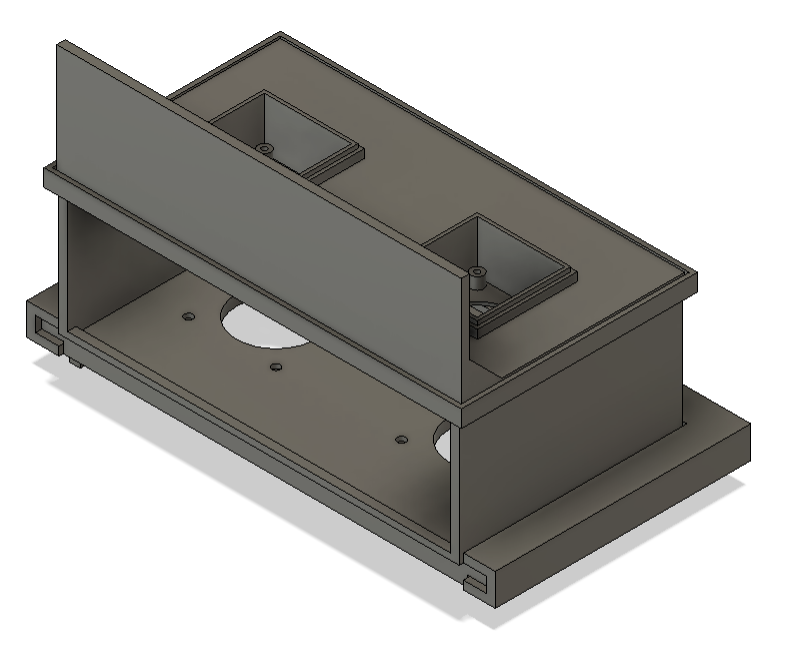
\includegraphics[width=0.75\textwidth]{Images/Figure 5.2.png}
    \caption[Experimental stereo rig configuration]{Experimental stereo rig configuration with fixed 100 mm baseline and rigid dual-camera mounting structure used for stereo image acquisition during the laboratory validation campaign.}
    \label{fig:figure5.2}
\end{figure}

\subsection{Processing unit and synchronization}

Stereo image acquisition, synchronization, and data management were performed using a Raspberry Pi Compute Module 5 (CM5). The platform was selected due to its support for dual MIPI CSI-2 camera interfaces, high data throughput, compact architecture, and compatibility with the stereo imaging hardware described in Section \ref{sec:camera_sensors}.
\\\\
The CM5 is based on a 64-bit quad-core Arm Cortex-A76 processor operating at 2.4 GHz and provides up to 16 GB of LPDDR4X memory, enabling simultaneous acquisition and management of high-resolution stereo image streams generated by the dual IMX477 camera system as illustrated in Figure \ref{fig:figure5.3} The platform also provides an architecture conceptually consistent with the distributed processing constraints anticipated for a future flight implementation.
\\\\
Because dedicated hardware triggering interfaces are not directly exposed through the standard development configuration, image synchronization was implemented through software-based acquisition control using the libcamera framework. The adopted synchronization strategy relies on low-latency sequential triggering between both cameras.
\\\\
For the quasi-static tether dynamics considered during laboratory testing, with deployment velocities below approximately $5~cm/s$, the resulting inter-frame delay remains sufficiently small to preserve stereo correspondence and maintain geometric consistency during reconstruction.
\newpage
\clearpage

\begin{figure}[!ht]
    \centering
    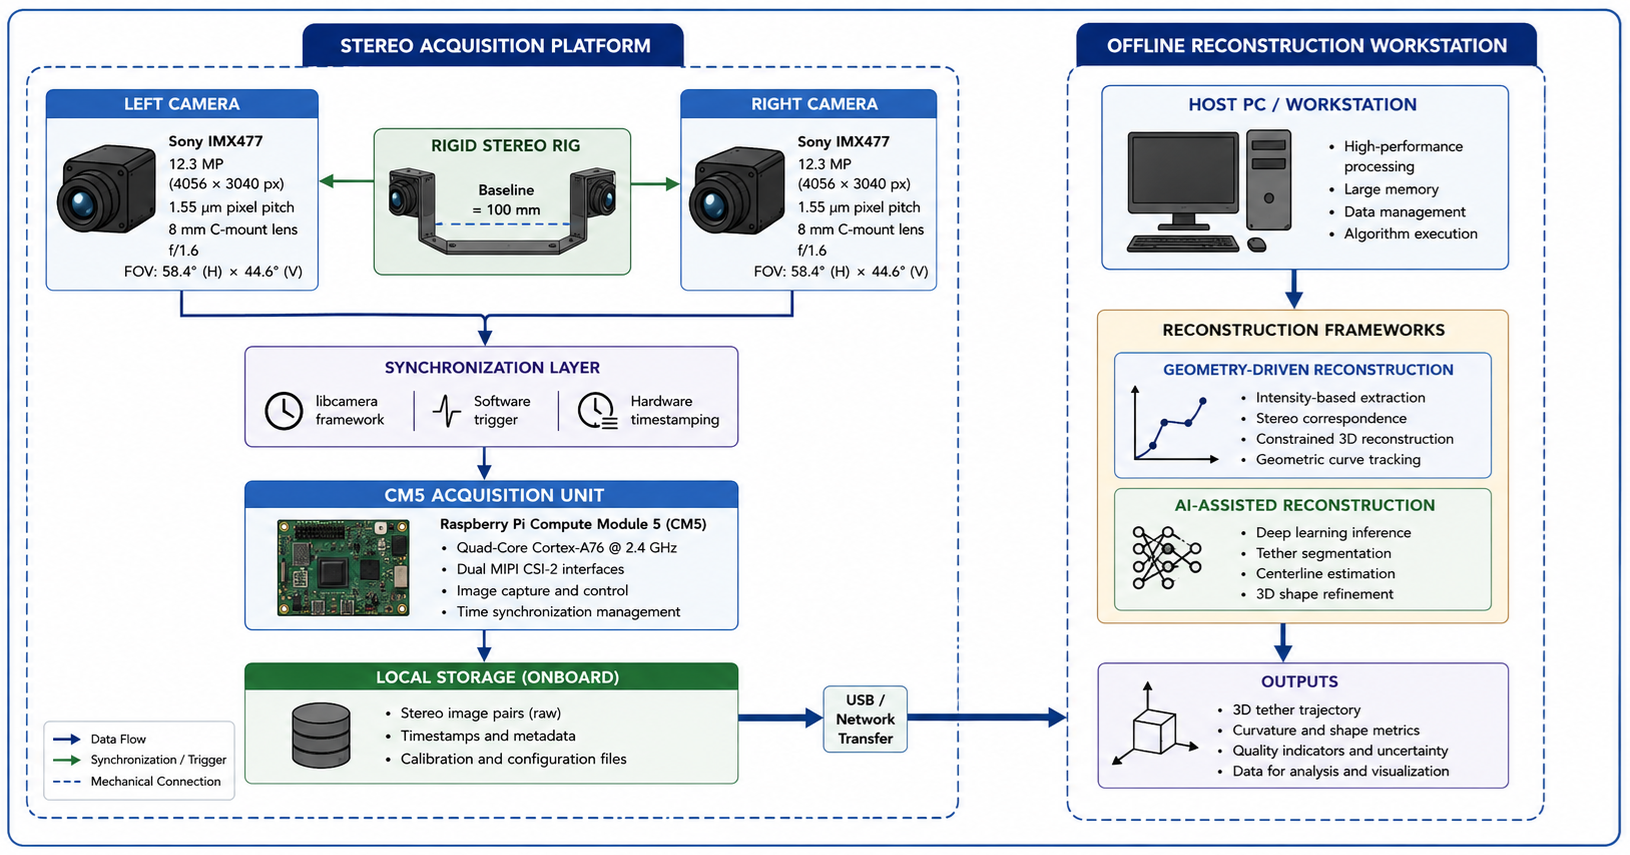
\includegraphics[width=\textwidth]{Images/Figure 5.3.png}
    \caption[Hardware architecture and data acquisition flow of the LINKU stereo vision system]{Hardware architecture and data acquisition flow of the LINKU stereo vision system. Dual IMX477 cameras acquire synchronized stereo imagery through the CM5 acquisition platform, which manages image capture, timestamping, and data transfer to the ground processing workstation.}
    \label{fig:figure5.3}
\end{figure}

\section{Experimental validation environment}
The experimental validation environment was developed to reproduce, under controlled laboratory conditions, the principal optical characteristics associated with orbital tether observation. The objective was not to replicate the complete space environment, but rather to emulate the visual conditions that directly influence tether detectability and stereo reconstruction performance.
\\\\
The experimental setup was therefore designed around the optical constraints identified in Chapter \ref{chap:theoretical-optical-analyses}, including low-texture backgrounds, high radiometric contrast, directional illumination, and sub-pixel tether visibility. Particular attention was given to controlling illumination conditions and background radiance in order to isolate the effects of geometric sampling and radiometric response on the reconstruction process.
\\\\
The resulting validation environment provides a repeatable platform for evaluating both conventional feature-based photogrammetry and the geometry-driven reconstruction methodology introduced in Chapter \ref{chap:experimental-processing-approaches}. By progressively reducing the availability of environmental texture while maintaining controlled imaging conditions, the setup enables systematic assessment of the transition from conventional image-based reconstruction toward radiometric and geometry-driven tether observation strategies.

\subsection{Validation philosophy and test scenarios}
The experimental validation strategy was organized around two complementary observation scenarios designed to evaluate reconstruction performance under progressively constrained visual conditions.
\\\\
The first scenario represents a terrestrial baseline environment in which conventional photogrammetry algorithms operate under favorable conditions. A volumetric target with clearly observable geometric features is imaged in the presence of environmental texture, enabling reliable feature extraction, stereo correspondence, and three-dimensional reconstruction. This scenario establishes a reference performance level for conventional image-based reconstruction techniques.
\\\\
The second scenario represents an orbital-like observation environment specifically designed for tether detection and reconstruction. In this configuration, environmental texture is intentionally minimized, background radiance is suppressed, and directional illumination is introduced to reproduce the high-contrast imaging conditions expected during orbital tether observation. Under these conditions, the target progressively transitions from a conventionally resolvable geometric object toward a radiometrically detectable structure, requiring reconstruction methods based on intensity localization, geometric continuity, and constrained stereo correspondence.
\\\\
Together, these two scenarios provide a controlled framework for evaluating the limitations of conventional feature-based photogrammetry and the applicability of geometry-driven reconstruction methods under conditions representative of the LINKU mission concept.

\subsection{Baseline terrestrial validation scenario}
The baseline terrestrial validation scenario was established to provide a reference environment in which conventional feature-based photogrammetry methods could operate under favorable visual conditions. This configuration verifies the nominal performance of stereo reconstruction algorithms before introducing the optical constraints associated with orbital tether observation.
\\\\
A volumetric object with well-defined geometric features was selected as the observation target. Unlike the tether considered in the LINKU mission, the object occupied a significant number of image pixels and contained sufficient visual texture to support reliable feature detection and matching. This configuration enabled the generation of stable stereo correspondences and three-dimensional reconstructions using standard photogrammetric techniques as presented in Figure \ref{fig:figure5.4}.
\\\\
To evaluate the influence of environmental texture on reconstruction performance, two imaging conditions were considered. In the first condition, the target was placed within a conventional laboratory environment containing visible background features. This configuration provided abundant visual references for feature extraction and served as the nominal reconstruction baseline.
\\\\
In the second condition, the same target was imaged against a uniform dark background with minimal environmental texture. Although the geometric characteristics of the object remained unchanged, the reduction of surrounding visual references allowed the sensitivity of conventional reconstruction methods to background texture availability to be assessed.
\\\\
These experiments establish a controlled reference for interpreting the results obtained in the orbital-like observation environment described in the following sections. By maintaining the same imaging hardware while progressively reducing scene texture, the setup enables direct comparison between conventional feature-based reconstruction and the geometry-driven methodologies developed for tether observation.
\newpage
\clearpage

\begin{figure}[!ht]
    \centering
    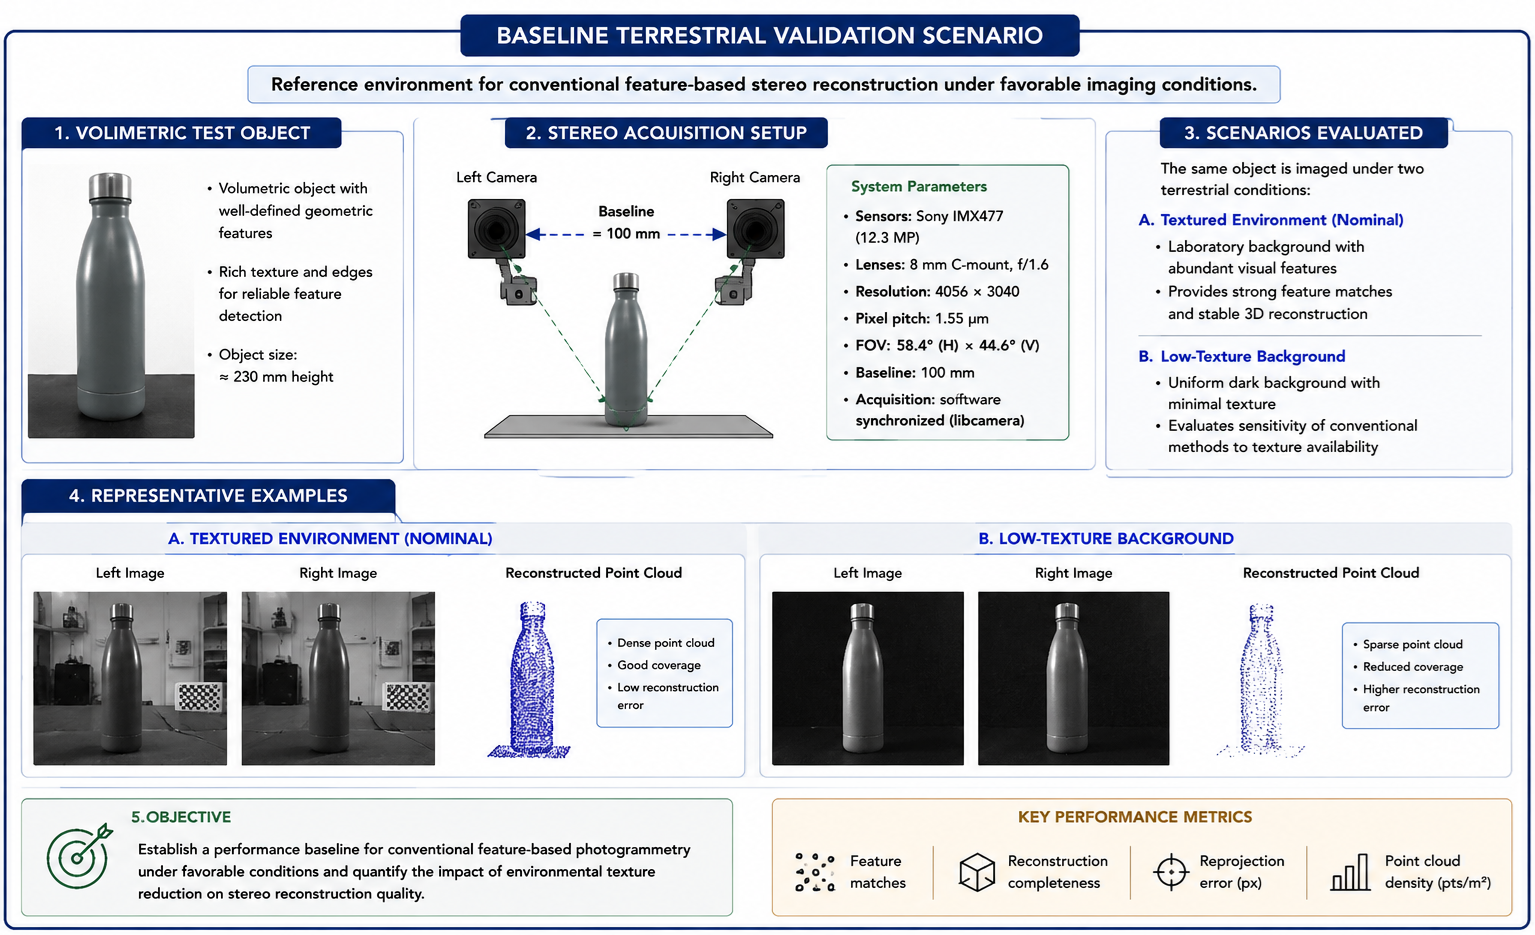
\includegraphics[width=\textwidth]{Images/Figure 5.4.png}
    \caption[Baseline terrestrial validation scenario.]{Baseline terrestrial validation scenario. A volumetric target with well-defined geometric features is observed under two controlled terrestrial conditions: a textured environment and a low-texture background. The comparison enables the evaluation of conventional feature-based stereo reconstruction performance and establishes a reference baseline against which the orbital-like tether observation scenarios can be assessed.}
    \label{fig:figure5.4}
\end{figure}

\subsection{Orbital-like observation environment}

The orbital-like observation environment was developed to reproduce, under controlled laboratory conditions, the principal optical characteristics associated with tether observation in orbit. Unlike the baseline terrestrial scenario described previously, this configuration intentionally minimizes environmental texture and background radiance while introducing highly directional illumination conditions.
\\\\
This environment will not replicate all aspects of the space environment, but rather to reproduce the visual constraints that directly affect tether detectability and stereo reconstruction performance. Particular emphasis was placed on generating conditions representative of low-texture scenes, high radiometric contrast, and sub-pixel target observation.
\\\\
The experimental configuration was designed to support the validation of the geometry-driven reconstruction methodology presented in Chapter \ref{chap:experimental-processing-approaches}. By progressively reducing the availability of conventional visual features, the setup enables evaluation of reconstruction strategies based on radiometric localization, geometric continuity, and constrained stereo correspondence.
\\\\
The orbital-like environment consists of three principal elements: a light-isolated enclosure, a directional illumination system, and a tether proxy representative of the expected mission target. Together, these elements provide a controlled platform for evaluating tether observation under conditions that approximate the optical challenges associated with orbital operation.

\subsubsection{Dark enclosure}
\label{subsub:Dark-enclosure}
A dedicated dark enclosure was constructed to isolate the experimental volume from ambient illumination and external visual references. The enclosure provides a controlled low-radiance environment intended to approximate the absence of background texture and stray light typically encountered during orbital observation.
\\\\
The enclosure was fabricated from laser-cut medium-density fiberboard (MDF) panels and has internal dimensions of approximately $600 mm \times 800 mm \times 500 mm$. All interior surfaces were coated with matte black paint to reduce diffuse reflections and suppress unwanted radiometric contributions from the surrounding environment.
\\\\
By minimizing background brightness and environmental texture, the enclosure increases the radiometric contrast between the observed target and the surrounding scene. This condition is particularly important for the evaluation of thin tether-like structures, whose detectability depends primarily on their radiometric response rather than on conventional texture-based image features.
\\\\
Figure \ref{fig:figure5.5} presents the dark enclosure used throughout the experimental validation campaign, including both the computer-aided design model and the fabricated implementation. The resulting environment provides a repeatable and controllable observation volume for the orbital-like experiments described in the following sections.

\begin{figure}[!ht]
    \centering
    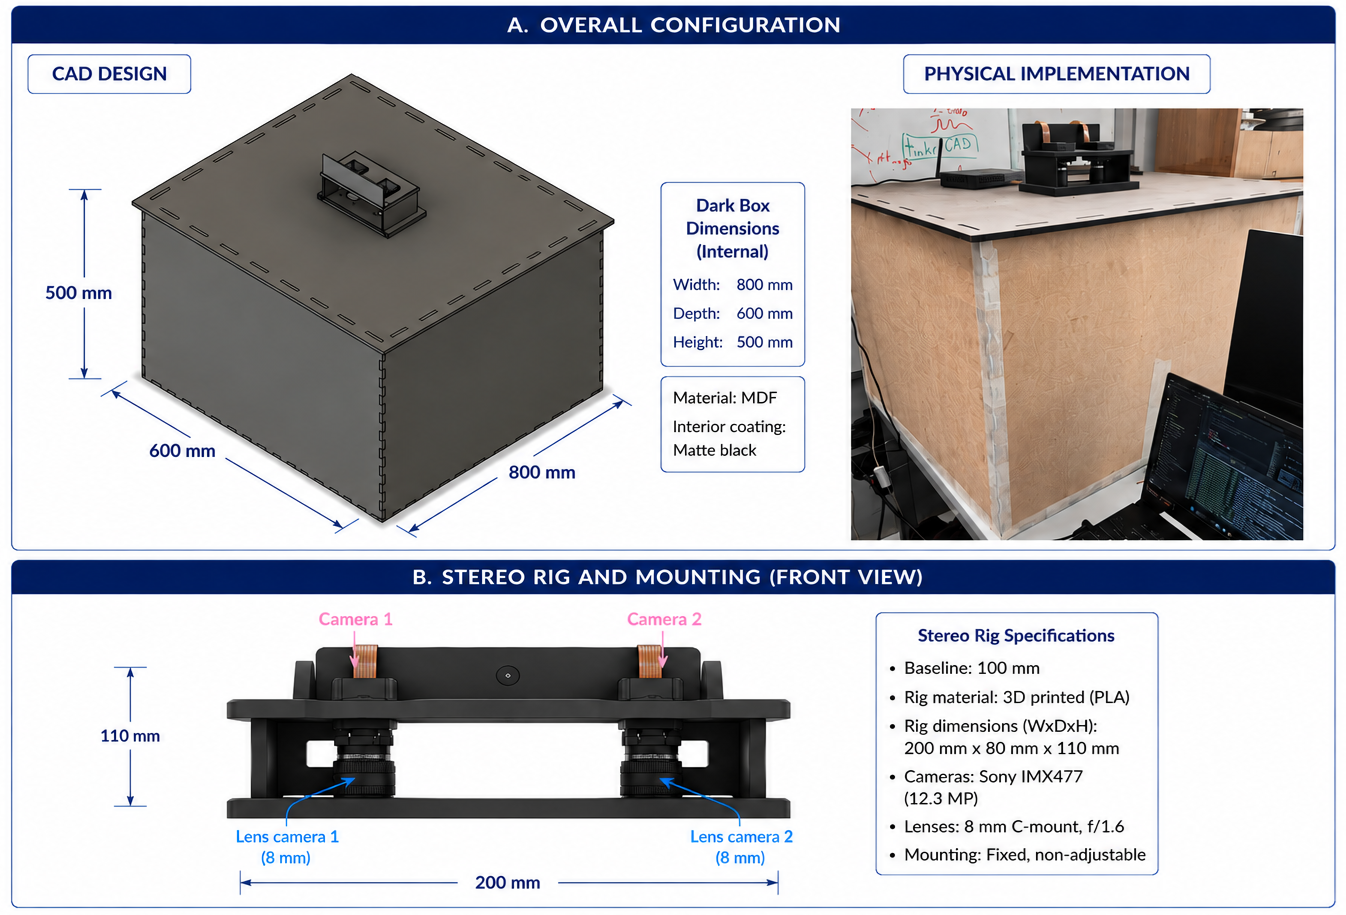
\includegraphics[width=\textwidth]{Images/Figure 5.5.png}
    \caption[Dark enclosure and stereo vision system configuration.]{Dark enclosure and stereo vision system configuration. (A) CAD model and physical implementation of the light-tight MDF enclosure used to reproduce low-texture, high-contrast orbital-like observation conditions. The enclosure provides an internal volume of approximately $800 mm \times 600 mm \times 500 mm$ and incorporates a matte-black interior coating to minimize reflections and background radiance. (B) Front view of the stereo rig used for image acquisition. The system consists of two Sony IMX477 cameras equipped with 8 mm C-mount lenses and mounted on a rigid structure with a fixed 100 mm stereo baseline, ensuring stable and repeatable stereo geometry during the experimental campaigns.}
    \label{fig:figure5.5}
\end{figure}

\subsubsection{Directional illumination system}

Reproducing the geometric characteristics of solar illumination within a laboratory-scale environment remains challenging. Under orbital conditions, the Sun behaves as an effectively collimated source with an apparent angular diameter of approximately $0.5^\circ$, producing nearly parallel rays, sharp shadow boundaries, and strong specular reflections.
\\\\
For the experimental campaign described in this work, a high-intensity directional LED source was employed to generate controlled illumination inside the dark enclosure. Although the source does not reproduce the full geometric characteristics of solar radiation, it provides sufficient radiometric contrast to evaluate tether detectability, intensity-based extraction, and centerline localization under high-contrast observation conditions.
\\\\
The adopted illumination strategy was intentionally designed to emphasize radiometric visibility effects rather than absolute solar irradiance levels. This approach is consistent with the primary objective of the validation campaign, namely the assessment of geometry-driven reconstruction performance under conditions where tether detectability becomes strongly dependent on illumination geometry.
\\\\
A similar challenge has been discussed by Sun et al. \cite{sun2022led}, who demonstrated that realistic solar simulation requires not only spectral matching but also controlled beam collimation, volumetric illumination uniformity, and directional consistency. Their LED-based solar simulator achieved approximately one solar constant irradiance with a beam divergence close to $\pm 3^\circ$, highlighting the importance of geometric illumination properties when reproducing solar observation conditions in laboratory environments.

\subsubsection{Tether proxy and observation target}

A tether proxy was employed to provide a controllable and repeatable representation of the tether structure considered in the LINKU mission concept. The proxy consisted of a thin cable with an external diameter of approximately 1 mm, selected to reproduce the small apparent dimensions and limited image occupancy characteristic of long-range tether observation.
\\\\
The target was positioned within the dark enclosure and observed under the directional illumination conditions described previously. By combining a low-texture background with a thin elongated structure, the experimental configuration creates imaging conditions in which target detectability becomes increasingly dependent on radiometric response rather than on conventional texture-based image features.
\\\\
Unlike the volumetric object used in the baseline terrestrial scenario, the tether proxy exhibits a highly anisotropic geometry with limited visual texture and a significantly reduced projected width within the image plane. These characteristics make the target representative of the reconstruction challenges addressed by the geometry-driven methodology developed in Chapter \ref{chap:experimental-processing-approaches}.
\\\\
The tether proxy therefore serves as the primary observation target for evaluating intensity-based extraction, centerline estimation, geometric curve tracking, stereo correspondence, and constrained three-dimensional reconstruction under orbital-like observation conditions.

\subsection{Representative experimental observations}

Representative observations acquired within the orbital-like validation environment are presented to illustrate the imaging conditions obtained using the experimental setup described in the previous sections. These observations provide qualitative verification that the combination of the dark enclosure, directional illumination system, and tether proxy successfully reproduces the principal optical characteristics required for geometry-driven tether reconstruction.
\\\\
Figure \ref{fig:figure5.6} shows a representative image of the 1 mm tether proxy acquired under directional illumination together with the corresponding extraction result. The observed image exhibits high radiometric contrast between the tether and the surrounding background, while maintaining minimal environmental texture within the field of view. This configuration is consistent with the orbital-like observation conditions discussed in Chapter \ref{chap:theoretical-optical-analyses}.

\begin{figure}[!ht]
    \centering
    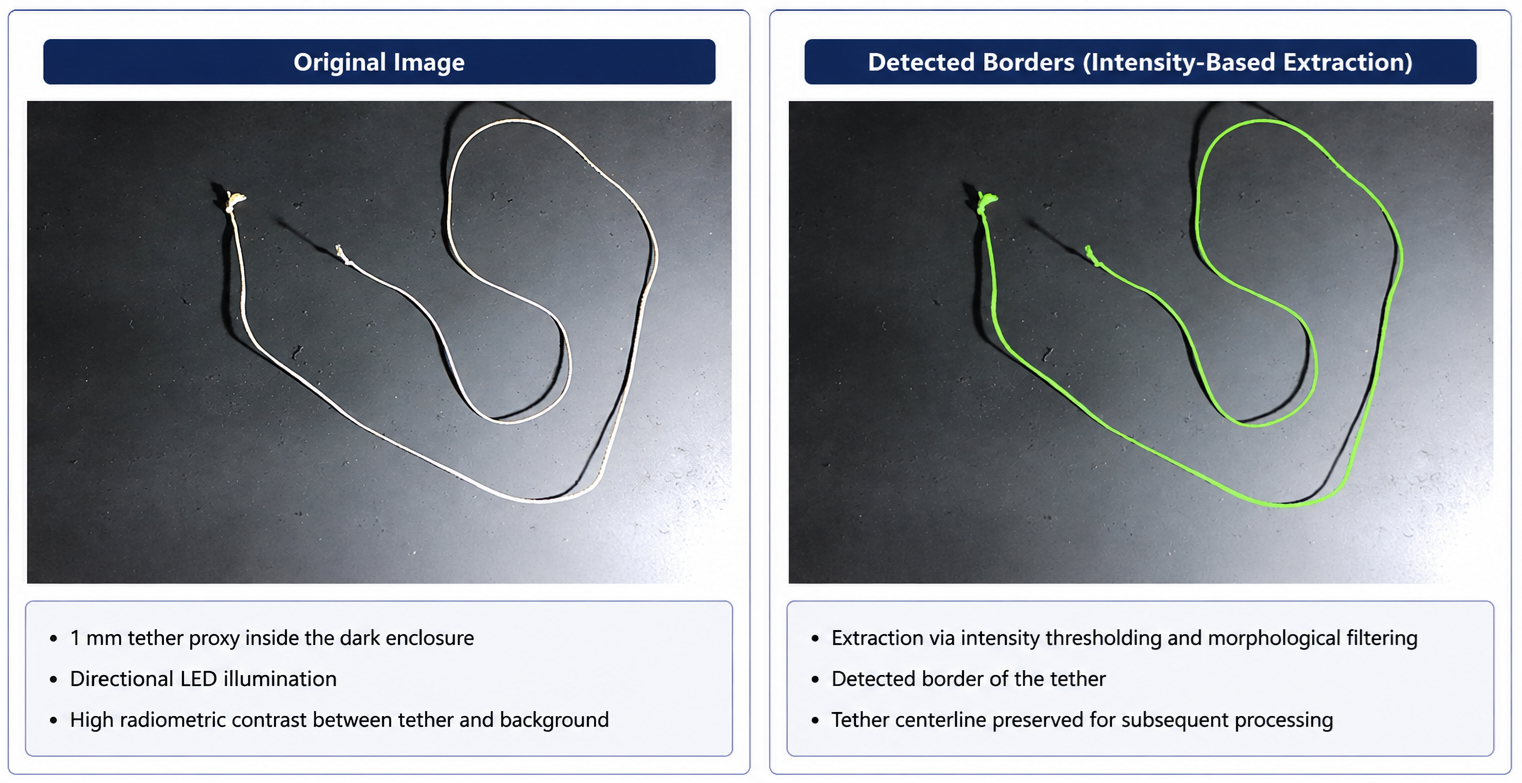
\includegraphics[width=\textwidth]{Images/Figure 5.6.png}
    \caption[Representative tether observation and intensity-based extraction.]{Representative tether observation and intensity-based extraction.}
    \label{fig:figure5.6}
\end{figure}

The extracted tether response demonstrates that the illumination and background suppression strategy provide sufficient target visibility for subsequent processing stages, including intensity-based extraction, centerline estimation, geometric curve tracking, and stereo correspondence. Although the tether occupies only a small fraction of the image area, its radiometric signature remains sufficiently distinguishable to support reliable geometric localization.
\\\\
These observations confirm that the experimental environment provides a suitable validation platform for evaluating the geometry-driven reconstruction methodology under controlled high-contrast conditions representative of orbital tether observation.

\section{Computational resources for offline reconstruction}

The experimental validation campaign generated stereo image datasets that were processed offline using dedicated computing resources. Separating image acquisition from reconstruction processing enabled systematic evaluation of the proposed methodologies while avoiding the computational and power constraints associated with embedded flight hardware.
\\\\
This approach provided full access to intermediate processing results, facilitating algorithm verification, parameter tuning, and quantitative performance assessment under the different observation scenarios described in the previous sections. Two complementary reconstruction approaches were evaluated throughout the study: a geometry-driven methodology based on radiometric and geometric constraints, and an exploratory AI-assisted reconstruction framework based on recent neural three-dimensional reconstruction techniques.

\subsection{Offline execution of the Geometry-driven reconstruction pipeline}

The geometry-driven reconstruction methodology developed in Section \ref{sec:Geometry-driven stereo reconstruction} was executed offline using the stereo image datasets acquired during the experimental validation campaign. This processing strategy enabled systematic evaluation of the proposed reconstruction framework while maintaining complete access to intermediate results for verification and analysis.
\\\\
The complete reconstruction workflow, summarized in Figure \ref{fig:figure4.3}, was applied consistently to all datasets acquired under both the baseline terrestrial scenario and the orbital-like observation environment. Using a common processing configuration ensured that reconstruction performance could be evaluated under different imaging conditions without introducing variations associated with algorithm implementation or parameter selection.
\\\\
All reconstruction experiments were executed on a workstation equipped with an Intel Core i9 processor and 64 GB of DDR4 memory. The computational requirements of the geometry-driven methodology remained relatively modest, allowing complete offline execution using conventional workstation hardware without dependence on dedicated high-end GPU acceleration.
\\\\
The computational environment was intentionally separated from the image acquisition platform described in Section \ref{sec:Hardware-architecture-data-acquisition}. This modular architecture allowed the experimental setup to focus on controlled data collection while providing sufficient flexibility for algorithm development, validation, and quantitative performance assessment under the different observation scenarios investigated in this work.

\subsection{AI-assisted reconstruction resources}

Exploratory AI-assisted reconstruction experiments were conducted to evaluate the potential applicability of recent neural three-dimensional reconstruction techniques to tether observation problems. Unlike the geometry-driven methodology, these approaches rely on learned scene representations and generative models that require greater computational resources.
\\\\
The AI-assisted experiments were executed using the same workstation platform employed for the geometry-driven reconstruction tasks, incorporating an Intel Core i9 processor, 64 GB of DDR4 memory, and an NVIDIA RTX 2070 GPU. For reconstruction models whose memory requirements exceeded the available local GPU resources, cloud-based execution was performed using Google Colab Pro environments equipped with NVIDIA V100 and A100 accelerators.
\\\\
The resulting computational requirements were higher than those associated with the geometry-driven reconstruction pipeline. While the geometry-driven methodology could be executed efficiently on conventional workstation hardware and remains compatible with future embedded implementations, the AI-assisted approaches required dedicated GPU acceleration and, in some cases, access to high-performance cloud computing resources.
\\\\
These observations reinforce the role of geometry-driven reconstruction as the primary operational strategy for the LINKU stereo vision system, while AI-assisted methods remain exploratory tools intended to support future research into reconstruction under visually ambiguous observation conditions.
